\documentclass[ ../main.tex]{subfiles}
\providecommand{\mainx}{..}
\begin{document}
\section{Error propagation through relational operators}
\label{sec:rel_algebra}
The relational operators of \cref{sec:relations} (selection, projection, and
join) build new relations from old ones. When the operands are random
approximate relations rather than exact relations, each operator induces a
\emph{derived} approximate relation whose membership test is a Boolean function
of the operand membership tests. Two questions then arise for every operator.
First, what are the derived error rates? Second, does the derived relation still
satisfy \emph{element-wise independence} (\cref{asm:ber_trial}), the axiom on
which the binomial error-count machinery of \cref{sec:prob_model} rests? The
answers depend on which random sources the outputs use. Selection restricts
the existing tests. Projection of an independent-tuple input preserves
independence, although its rates can vary by fiber. A join can reuse an input
source in several outputs and thereby correlate them. Canonical representations
also share sources; projection of such a representation need not preserve
tuple independence.

Throughout, $\Relation{R}$ and $\Relation{S}$ are exact relations of objective
interest, approximated by Bernoulli relations
$\ARelation{R}[\fprate_R][\tprate_R]$ and $\ARelation{S}[\fprate_S][\tprate_S]$
over their respective tuple universes, with $\tprate_R = 1 - \fnrate_R$ the
true-positive rate and $\fnrate_R$ the false-negative rate (likewise for
$\Relation{S}$). Except in the explicitly identified source-sharing extension
below, the two approximations are independent of each other and each satisfies
\cref{asm:ber_trial}: distinct tuple trials are mutually independent, with
common rates within each exact membership class. This does not include a
self-join using the same construction as both operands. Any predicate appearing in an operator
(the selection predicate $\theta$, the join condition, the equality of projected
attribute values) is an \emph{exact} predicate on known tuple values: it carries
no randomness. The only randomness in any derived relation is inherited from the
operand membership tests.

\subsection{Selection}
\label{sec:select}
Selection $\Selection_\theta$ keeps exactly those tuples of a relation that
satisfy a predicate $\theta$ on their values. Because $\theta$ is exact, the
approximate selection is nothing more than the operand relation read on a
smaller universe.

\begin{theorem}[Selection is rate-transparent]
\label{thm:select}
Let $\theta$ be an exact predicate on the tuples of the universe
$\Set{U} = \Set{X}[1] \times \cdots \times \Set{X}[n]$, and let
$\ARelation{R}[\fprate_R][\tprate_R]$ approximate $\Relation{R} \subseteq \Set{U}$.
Then the approximate selection $\Selection_\theta(\ARelation{R})$ is the
restriction of $\ARelation{R}$ to the sub-universe
$\Set{U}_\theta = \SetBuilder{t \in \Set{U}}{\theta(t)}$. It is a Bernoulli
relation of $\Selection_\theta(\Relation{R})$ over $\Set{U}_\theta$ with the
\emph{same} rates $(\fprate_R, \tprate_R)$, and element-wise independence
(\cref{asm:ber_trial}) is preserved.
\end{theorem}
\begin{proof}
A tuple $t \in \Set{U}_\theta$ is accepted by $\Selection_\theta(\ARelation{R})$
if and only if it is accepted by $\ARelation{R}$, since $\theta(t)$ holds with
certainty and contributes no further test. For $t \in \Set{U}_\theta$ the
conditioning on the exact relation is unchanged,
\begin{equation}
    \Prob{t \in \Selection_\theta(\ARelation{R}) \Given t \notin \Relation{R}}
    = \Prob{t \in \ARelation{R} \Given t \notin \Relation{R}} = \fprate_R\,,
\end{equation}
and likewise the true-positive rate on $\Set{U}_\theta$ is $\tprate_R$.
Restricting the universe selects a sub-collection of the original Bernoulli
trials; it neither rescales any per-tuple rate nor introduces any coupling
between distinct trials. Thus independence and the rates within each exact
membership class are preserved.
\end{proof}

Selection preserves this marginal-rate partition; it does not turn a two-rate
model into a one-rate model. If the output is instead viewed over the original
universe $\Set{U}$, tuples outside $\Set{U}_\theta$ are deterministic negatives.
For a source-sharing input, selection retains any dependence among the selected
tuples.

\subsection{Projection}
\label{sec:project}
Projection $\Proj_Y$ onto an attribute subset $Y$ drops the remaining columns.
Several distinct tuples of $\Relation{R}$ can agree on their $Y$-components and so
collapse onto a single projected tuple. The pre-image of a projected tuple is its
\emph{fiber}.

\begin{definition}[Fiber]
\label{def:fiber}
For a projected tuple $s$ in the target universe of $\Proj_Y$, the \emph{fiber}
of $s$ is the set of operand tuples that project onto it,
\begin{equation}
    \fiber(s) = \SetBuilder{t \in \Set{U}}{ t|_Y = s }\,,
\end{equation}
and its size is the \emph{fan-in} $k(s) = \Card{\fiber(s)}$. We use the image
of the candidate universe as the target universe, so every fiber considered is
nonempty. A target tuple with an empty fiber is rejected deterministically.
\end{definition}

A projected tuple $s$ is accepted by the approximate projection exactly when at
least one tuple of its fiber is accepted by $\ARelation{R}$: projection is a
logical \textsc{or} over the fiber. Because the fiber tuples are \emph{distinct}
elements of $\Set{U}$, their $\ARelation{R}$-memberships are independent
(\cref{asm:ber_trial}), and the \textsc{or} composes their rates multiplicatively
on the complementary event.

\begin{theorem}[Projection amplifies the false-positive rate]
\label{thm:project}
Let $\ARelation{R}[\fprate_R][\tprate_R]$ approximate $\Relation{R}$, and let
$s$ be a projected tuple under $\Proj_Y$ with fiber $\fiber(s)$ of size $k(s)$.
The approximate projection $\Proj_Y(\ARelation{R})$ accepts $s$ if and only if
some tuple of $\fiber(s)$ is accepted by $\ARelation{R}$. Then:
\begin{enumerate}[(i)]
    \item If $s \notin \Proj_Y(\Relation{R})$, every fiber tuple is a true
    negative, and $s$ is a false positive of the projection unless all $k(s)$
    independent trials miss:
    \begin{equation}
        \fprate_\Proj(s) = 1 - (1-\fprate_R)^{k(s)} \;\geq\; \fprate_R\,.
    \end{equation}
    \item If $s \in \Proj_Y(\Relation{R})$, say $j \geq 1$ of the fiber tuples
    are true members of $\Relation{R}$ and the remaining $k(s)-j$ are non-members,
    then $s$ is correctly accepted unless every fiber trial misses:
    \begin{equation}
        \tprate_\Proj(s) = 1 - (1-\tprate_R)^{j}\,(1-\fprate_R)^{k(s)-j}
        \;\geq\; \tprate_R\,.
    \end{equation}
\end{enumerate}
The false-positive rate is amplified by the fan-in, and the true-positive rate is
boosted, because a non-member fiber tuple can itself false-positive and so rescue
the projection of a genuine member.
\end{theorem}
\begin{proof}
The acceptance event for $s$ is the union, over $t \in \fiber(s)$, of the
acceptance events $\{ t \in \ARelation{R} \}$. Distinct tuples have independent
memberships (\cref{asm:ber_trial}), so the probability that the union fails is the
product of the per-tuple failure probabilities.

If $s \notin \Proj_Y(\Relation{R})$ then no tuple of $\fiber(s)$ lies in
$\Relation{R}$, so each of the $k(s)$ tuples is accepted independently with
probability $\fprate_R$ and missed with probability $1-\fprate_R$. The projection
misses $s$ with probability $(1-\fprate_R)^{k(s)}$, giving
\begin{equation}
    \fprate_\Proj(s)
    = 1 - \prod_{t \in \fiber(s)} \Prob{t \notin \ARelation{R} \Given t \notin \Relation{R}}
    = 1 - (1-\fprate_R)^{k(s)}\,.
\end{equation}
If $s \in \Proj_Y(\Relation{R})$ then at least one fiber tuple lies in
$\Relation{R}$; partition the fiber into the $j \geq 1$ members, each missed with
probability $1-\tprate_R$, and the $k(s)-j$ non-members, each missed with
probability $1-\fprate_R$. By independence the projection misses $s$ with
probability $(1-\tprate_R)^{j}(1-\fprate_R)^{k(s)-j}$, so
\begin{equation}
    \tprate_\Proj(s) = 1 - (1-\tprate_R)^{j}\,(1-\fprate_R)^{k(s)-j}\,.
\end{equation}
Both bounds follow since each factor lies in $[0,1]$: including additional
factors can only decrease the product and increase the complementary rate.
\end{proof}

The rate formulas depend on $s$ only through its fan-in $k(s)$ (and, for true
members, the member count $j$), which varies from one projected tuple to the next.
This is the structural heart of projection. \Cref{fig:proj_fpr} plots the
amplified false-positive rate $1-(1-\fprate)^{k}$ against the fan-in $k$ for three
operand rates, making the growth with $k$ explicit: even a modest operand rate is
driven up steeply once several tuples share a projected image.

\begin{figure}[ht]
    \centering
    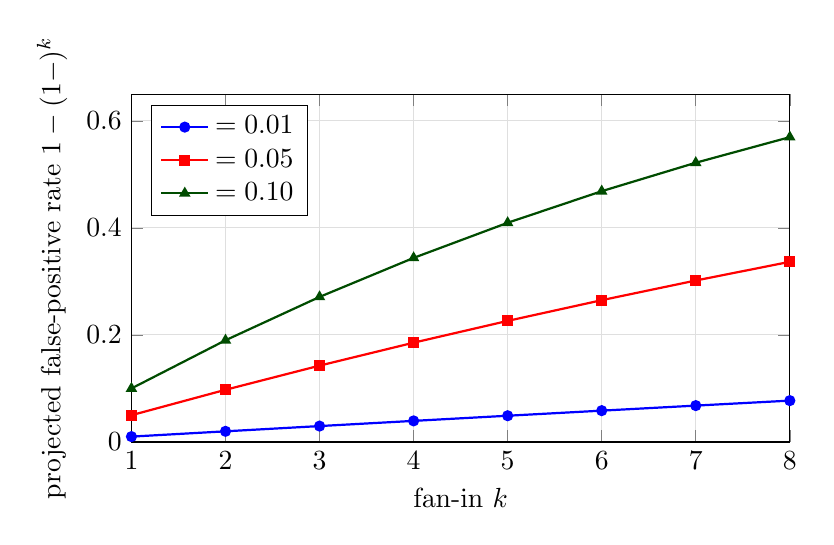
\begin{tikzpicture}
        \begin{axis}[
            width=0.82\linewidth,
            height=6cm,
            xlabel={fan-in $k$},
            ylabel={projected false-positive rate $1-(1-\fprate)^{k}$},
            xmin=1, xmax=8,
            ymin=0, ymax=0.65,
            xtick={1,2,3,4,5,6,7,8},
            legend pos=north west,
            legend cell align={left},
            grid=major,
            grid style={gray!25},
            mark size=1.6pt,
        ]
        \addplot[mark=*, thick, blue]
            coordinates {
                (1,0.010000) (2,0.019900) (3,0.029701) (4,0.039404)
                (5,0.049010) (6,0.058520) (7,0.067935) (8,0.077255)
            };
        \addlegendentry{$\fprate = 0.01$}
        \addplot[mark=square*, thick, red]
            coordinates {
                (1,0.050000) (2,0.097500) (3,0.142625) (4,0.185494)
                (5,0.226219) (6,0.264908) (7,0.301663) (8,0.336580)
            };
        \addlegendentry{$\fprate = 0.05$}
        \addplot[mark=triangle*, thick, black!70!green]
            coordinates {
                (1,0.100000) (2,0.190000) (3,0.271000) (4,0.343900)
                (5,0.409510) (6,0.468559) (7,0.521703) (8,0.569533)
            };
        \addlegendentry{$\fprate = 0.10$}
        \end{axis}
    \end{tikzpicture}
    \caption{False-positive amplification under projection
    (\cref{thm:project}). A projected tuple whose fiber has fan-in $k$ acquires
    false-positive rate $1-(1-\fprate)^{k}$, the probability that at least one of
    its $k$ independent fiber trials fires. The rate climbs with the fan-in and
    approaches $1$ for fixed $\fprate>0$, so projection onto an attribute subset with large fibers can
    turn a small operand false-positive rate into a substantial one.}
    \label{fig:proj_fpr}
\end{figure}

\begin{theorem}[Projection of independent tuples]
\label{thm:project_order}
Under \cref{asm:ber_trial}, distinct projected tuples have mutually independent
membership indicators. A sufficient partition into homogeneous marginal-rate
blocks is given by the attained pairs $(k(s),j(s))$, where
$j(s)=\Card{\fiber(s)\cap\Relation{R}}$. The acceptance rate on such a block is
\begin{equation}
 1-(1-\tprate_R)^{j(s)}(1-\fprate_R)^{k(s)-j(s)}.
\end{equation}
The block is negative when $j(s)=0$ and positive otherwise. Different pairs may
give the same rate, so the number of distinct profiles need not equal the
minimal number of rate blocks.
\end{theorem}
\begin{proof}
If $s \neq s'$ then $t|_Y = s$ and $t|_Y = s'$ cannot both hold, so
$\fiber(s) \cap \fiber(s') = \EmptySet$. The acceptance of $s$ is a function of
the trials indexed by $\fiber(s)$ alone. The whole family of fibers is disjoint,
so functions of their mutually independent trial sets are mutually independent.
The rate formula and its constancy on the stated blocks follow from
\cref{thm:project}.
\end{proof}

On a full Cartesian candidate universe, coordinate projection has constant
fan-in equal to the product of the discarded domain sizes. Nonuniform fan-in
can arise after restricting that universe, for example by selection. In either
case the true-member count $j(s)$ can vary.

\begin{corollary}[Uniform fiber profiles]
\label{cor:uniform_fanin}
If every fiber has size $k$, negative projected tuples have common
false-positive rate $1-(1-\fprate_R)^k$. If in addition every positive fiber
has the same true-member count $j_\star\ge1$, those tuples have common
true-positive rate
$1-(1-\tprate_R)^{j_\star}(1-\fprate_R)^{k-j_\star}$.
Uniform fan-in alone need not give a common true-positive rate.
\end{corollary}

For example, at $(\fprate_R,\tprate_R)=(0.05,0.90)$, fibers with
$(k,j)=(3,1)$ and $(3,2)$ have true-positive rates $0.90975$ and $0.9905$.
The rates use the same two input parameters but differ because the exact fiber
profiles differ. In the collection's terminology~\cite{bernoulliSets},
\emph{model order} concerns the rate partition, while the number of free
channel parameters and the independence structure are separate questions.

\paragraph{Projection after source sharing.}
The preceding independence statement cannot be applied unchanged after a
canonical representation identifies different tuples with the same source.
Let $A_s$ be the set of distinct source IDs appearing in the fiber of $s$,
so its output indicator is $Y_s=\bigvee_{i\in A_s}Z_i$. This setting covers
canonical membership bits, not arbitrary Boolean formulas already produced by
a join.

\begin{theorem}[Projection with shared independent sources]
\label{thm:project_sources}
Under \cref{asm:source_model}, assume the distinct source bits $Z_i$ are
mutually independent, with $\Prob{Z_i=1}=p_i$. For a source set $C$ put
$q_C=\prod_{i\in C}(1-p_i)$, with $q_{\EmptySet}=1$. Then
\begin{align}
 \Prob{Y_s=1}&=1-q_{A_s},\\
 \operatorname{Cov}(Y_s,Y_t)
 &=q_{A_s\setminus A_t}\,q_{A_t\setminus A_s}\,
   q_{A_s\cap A_t}(1-q_{A_s\cap A_t}).
\end{align}
If every participating source has $0<p_i<1$, the projected indicators are
mutually independent exactly when their nonempty source supports are pairwise
disjoint.
\end{theorem}
\begin{proof}
The projection rejects exactly when all its distinct sources reject, proving
the first formula. Complementation of both indicators preserves covariance, so
\begin{equation}
 \operatorname{Cov}(Y_s,Y_t)=q_{A_s\cup A_t}-q_{A_s}q_{A_t}.
\end{equation}
Factoring over the three disjoint sets $A_s\setminus A_t$,
$A_t\setminus A_s$, and $A_s\cap A_t$ gives the result. At interior rates
any shared source makes the covariance strictly positive. Conversely, disjoint
supports give functions of disjoint independent source sets, hence mutual
independence. Empty supports produce constant-zero indicators.
\end{proof}

At boundary rates an overlapping support can still give zero covariance; the
formula remains valid, but the disjointness criterion needs the interior-rate
assumption. For a two-tuple candidate universe
$\{\Pair{a}{b},\Pair{b}{a}\}$, $a\ne b$, a symmetry-preserving canonical test
uses one source $Z$ for both tuples. Projection onto the first coordinate has
disjoint tuple fibers but identical source supports. Its two outputs both
equal $Z$ and have covariance $p(1-p)$. Distinct tuples are therefore not
necessarily distinct random trials.

\subsection{Join}
\label{sec:join}
The join $\Relation{R} \Join \Relation{S}$ pairs a tuple $r$ of $\Relation{R}$
with a tuple $s$ of $\Relation{S}$ whenever they agree on the common attributes,
and a join tuple is a member if and only if both operand tuples are members
(the join condition on values is exact). The join is therefore a logical
\textsc{and} of two independent operand tests. The per-tuple rates follow the
intersection (\textsc{and}) rules of two Bernoulli sets, which are proved in the
composition paper.

\begin{theorem}[Join error rates]
\label{thm:join}
Let $\ARelation{R}[\fprate_R][\tprate_R]$ and
$\ARelation{S}[\fprate_S][\tprate_S]$ be independent approximations of
$\Relation{R}$ and $\Relation{S}$. For a candidate output tuple $(r,s)$ whose
component values satisfy the exact join condition, distinguish the exact
memberships of $r$ in $\Relation{R}$ and $s$ in $\Relation{S}$:
\begin{enumerate}[(i)]
    \item If $(r,s) \in \Relation{R} \Join \Relation{S}$ (so $r \in \Relation{R}$
    and $s \in \Relation{S}$), the join tuple is missed exactly when either
    operand misses its tuple, giving the intersection false-negative rate
    \begin{equation}
        \fnrate_\Join = 1 - \tprate_R \tprate_S
                      = \fnrate_R + \fnrate_S - \fnrate_R \fnrate_S\,.
    \end{equation}
    \item If $(r,s) \notin \Relation{R} \Join \Relation{S}$, the false-positive
    rate depends on \emph{which} operand fails. When both operand tuples are
    absent ($r \notin \Relation{R}$ and $s \notin \Relation{S}$), the join
    false-positives only if both operands false-positive, with probability
    \begin{equation}
        \fprate_R \fprate_S\,,
    \end{equation}
    the sparse, both-absent corner of the three-region weighted intersection
    false-positive rate. When only one operand tuple is absent, that tuple must
    false-positive while the present tuple is correctly accepted, contributing the
    absent operand's false-positive rate weighted by the present operand's
    true-positive rate.
\end{enumerate}
If a specified distribution on negative candidate outputs assigns weights
$w_{01},w_{10},w_{00}$ to the three exact-membership regions, its average
false-positive rate is
\begin{equation}
 w_{01}\fprate_R\tprate_S+
 w_{10}\tprate_R\fprate_S+
 w_{00}\fprate_R\fprate_S,\qquad
 w_{01}+w_{10}+w_{00}=1.
\end{equation}
This is the weighted intersection rate~\cite{bernoulliComposition}; without a
query distribution or region counts, the three pointwise regimes remain
distinct.
\end{theorem}
\begin{proof}
A join tuple $(r,s)$ is reported by $\ARelation{R} \Join \ARelation{S}$ if and
only if $r \in \ARelation{R}$ and $s \in \ARelation{S}$, since the value-level
join condition is exact. The two operand tests are independent, by the
\emph{inter-relation} independence assumed at the start of this section, a
standing assumption distinct from the per-tuple independence of
\cref{asm:ber_trial}.

For (i), with $r \in \Relation{R}$ and $s \in \Relation{S}$, the tuple is correctly
reported with probability $\tprate_R \tprate_S$ and missed otherwise, so
\begin{equation}
    \fnrate_\Join = 1 - \tprate_R \tprate_S
                  = 1 - (1-\fnrate_R)(1-\fnrate_S)
                  = \fnrate_R + \fnrate_S - \fnrate_R \fnrate_S\,,
\end{equation}
which is the false-negative rule for the intersection of two Bernoulli
sets~\cite{bernoulliComposition}.

For (ii), $(r,s)$ is a non-member when at least one operand tuple is a non-member,
and it is reported only if \emph{both} operand tests fire. If both tuples are
non-members the two firings are false positives, occurring independently with
probability $\fprate_R \fprate_S$. If exactly one tuple is a non-member, say
$r \notin \Relation{R}$ while $s \in \Relation{S}$, then reporting requires a
false positive on $r$ (probability $\fprate_R$) and a true positive on $s$
(probability $\tprate_S$), for $\fprate_R \tprate_S$; symmetrically
$\tprate_R \fprate_S$ in the other one-absent region. The average
false-positive rate under the specified query distribution is the weighted average of these three regions,
which is exactly the intersection false-positive rate
of~\cite{bernoulliComposition}. The value $\fprate_R\fprate_S$ alone is only
the both-absent corner. It understates the average when a one-absent region
has positive weight and a strictly larger acceptance rate; that comparison
requires the corresponding true-positive rate to exceed the false-positive
rate.
\end{proof}

Per-tuple, then, the join is well behaved: every output tuple has a well-defined
false-negative and false-positive rate. The subtlety is not in the marginal rates
but in the \emph{dependence} among output tuples.

\begin{theorem}[Joins can destroy element-wise independence]
\label{thm:join_dependence}
Consider compatible output tuples $(r,s_1)$ and $(r,s_2)$, with $s_1\ne s_2$,
and put $a=\Prob{r\in\ARelation{R}}$ and
$b_i=\Prob{s_i\in\ARelation{S}}$. Under the standing independent-input
assumptions, their indicators have covariance
\begin{equation}
 a(1-a)b_1b_2.
\end{equation}
It is strictly positive when $0<a<1$ and $b_1b_2>0$, proving that joins do not
preserve tuple independence in general. A join whose output tuples use
pairwise disjoint input trials does preserve independence.
\end{theorem}
\begin{proof}
Consider two output tuples $(r, s_1)$ and $(r, s_2)$ that share the same
left component $r$, with $s_1 \neq s_2$. Both acceptance events contain the
\emph{same} trial $\{ r \in \ARelation{R} \}$ as a conjunct:
\begin{equation}
    \{ (r,s_1) \in \ARelation{R} \Join \ARelation{S} \}
    = \{ r \in \ARelation{R} \} \cap \{ s_1 \in \ARelation{S} \}\,,
\end{equation}
and likewise for $(r,s_2)$ with $s_2$. Write $A = \{ r \in \ARelation{R} \}$ with
$\Prob{A} = a$, and let $B_i = \{ s_i \in \ARelation{S} \}$ be independent of $A$
and of each other. Then the two output indicators are $\SetIndicator{A \cap B_1}$ and
$\SetIndicator{A \cap B_2}$, with
\begin{equation}
    \Prob{(r,s_1), (r,s_2) \text{ both accepted}} = a\,\Prob{B_1}\Prob{B_2}\,,
\end{equation}
whereas the product of the marginals is
$a\Prob{B_1}\cdot a\Prob{B_2}=a^2b_1b_2$. Their difference is the stated
covariance. Under its strict-positivity conditions, the joint probability is
$1/a$ times the product of marginals and the two outputs are dependent.
The disjoint-input case follows because the output indicators are functions
of disjoint independent trial sets.
\end{proof}

At $a=0$ or $a=1$, or when a partner never accepts, this shared-component
covariance is zero. The theorem establishes a source-reuse mechanism, not a
claim that every join produces dependence. Downstream formulas that assume
independence over the output tuples (for
instance, the probability that an entire query result is error-free, computed as a
product of per-tuple correctness probabilities) are therefore not valid for a raw
join in general: the shared-component dependence must be carried explicitly. The marginal
rates of \cref{thm:join} are still exactly right for any \emph{single} output
tuple, and for the false-positive count of a join one may still take expectations
tuple by tuple (linearity of expectation does not require independence); it is the
higher moments and the all-correct probability that feel the correlation.

\subsection{A worked example with rates}
\label{sec:rel_example}
Consider the exact relations
\begin{equation}
 \Relation{A}=\{\Pair{a}{c}\}\subseteq\Set{X}\times\Set{Y},\qquad
 \Relation{B}=\{\Pair{c}{b},\Pair{c}{d}\}
 \subseteq\Set{Y}\times\Set{Z},\qquad b\ne d.
\end{equation}
Their join on $\Set{Y}$ contains $\Tuple{a,c,b}$ and $\Tuple{a,c,d}$.
Give each operand an independent-tuple approximation, and take the two
constructions to be independent, with illustrative rates
\begin{equation}
 \fprate=0.05,\qquad \fnrate=0.10,\qquad \tprate=0.90.
\end{equation}

\begin{example}
\emph{Single-tuple error and shared-input dependence.}
Each true join tuple requires two true source memberships, so its
true-positive rate is $\tprate^2=0.81$ and its false-negative rate is
$1-\tprate^2=0.19$. For a compatible candidate whose two source tuples
are both absent, the false-positive rate is instead
$\fprate^2=0.0025$.

The two true output tuples share the trial on $\Pair{a}{c}$ but have
distinct right-hand trials. Consequently,
\begin{align}
 \Prob{\text{both accepted}}&=\tprate^3=0.729,\\
 \Prob{\text{first}}\Prob{\text{second}}&=\tprate^4=0.6561.
\end{align}
Their covariance is $0.0729$, and their joint acceptance probability is
$1/\tprate\approx1.11$ times the product of marginals, as predicted by
\cref{thm:join_dependence}.

\emph{Projection needs candidate fibers.}
Projection onto $\Set{X}\times\Set{Z}$ sends the two displayed true rows to
$\Pair{a}{b}$ and $\Pair{a}{d}$. These distinct images do not establish
singleton candidate fibers: the ambient domains can supply additional
candidate tuples outside the exact join. Moreover, join outputs already
share sources, so \cref{thm:project} cannot be applied by treating each join
row as an independent trial.

For a separate independent-tuple input $\ARelation{T}$, a negative projected
tuple with three candidate tuples in its fiber has false-positive rate
\begin{equation}
 \fprate_\Proj=1-(1-\fprate)^3=1-0.95^3=0.142625.
\end{equation}
This is nearly triple the operand rate. The calculation applies to that
independent fiber, not automatically to a fiber of the dependent join above.
\end{example}

A full join-then-project calculation must retain the original source identities
in its Boolean query formula. The contracts of \cref{sec:query_contracts}
address such derived outputs.

\subsection{Independent-trial validation}
\label{sec:rel_validation}
The closed-form rates above are checked by direct Monte Carlo simulation in the
script \texttt{validate.py} (in the paper's \texttt{code/} directory). Each
approximate relation is realized as one independent Bernoulli trial per tuple: a
genuine member is reported with probability $\tprate = 1 - \fnrate$ and a
non-member with probability $\fprate$, exactly the per-tuple law of
\cref{asm:ber_trial}. The script then assembles the operator outputs (the fiber
\textsc{or} of a projection, the operand \textsc{and} of a join, the ordered-pair
\textsc{or} of a symmetric closure) and estimates each reported rate over
$2\times 10^{6}$ trials, using seed $20260608$. The same harness checks
selected invariant results of \cref{sec:invariants}: reflexivity, symmetry,
single-valuedness for defined and undefined keys, OR-closure at actual orbit
sizes one through four, the canonical test's base rates
(\cref{sec:closure_dichotomy}), the deletion repair's retained-true-value
rate, and the deterministic
$\lceil \log_2 k \rceil$-pass transitivity cascade, including the non-power-of-two
path lengths that exercise the ceiling. \Cref{tbl:validation} transcribes the headline
comparisons at the illustrative rates $\fprate = 0.05$, $\fnrate = 0.10$
($\tprate = 0.90$). The largest absolute discrepancy among the fitted rows is
$0.000429$, below the script's $0.005$ tolerance. Separate finite-enumeration
checks in \texttt{test\_math\_validation.py} exercise the corrected
single-valuedness law, variable orbit sizes, source-overlap covariance, and
boundary rates zero and one.

\begin{table}[ht]
    \centering
    \caption{Analytical rates versus Monte Carlo estimates ($2\times 10^{6}$
    trials per row, $\fprate = 0.05$, $\fnrate = 0.10$, $\tprate = 0.90$;
    \texttt{code/validate.py}). The projection rows exhibit the fan-in
    amplification of \cref{thm:project}; the join rows exhibit both the
    intersection false-negative rate of \cref{thm:join} and the
    independence-failure correlation of \cref{thm:join_dependence}; the closure
    rows distinguish off-diagonal pairs from singleton diagonal trials in
    \cref{thm:symmetric_closure}.}
    \label{tbl:validation}
    \small
    \begin{tabular}{@{}l l r@{\hspace{1.4em}}r@{}}
        \toprule
        result & formula & analytical & empirical\\
        \midrule
        Projection $\fprate$, $k=2$ & $1-(1-\fprate)^2$ & $0.097500$ & $0.097320$\\
        Projection $\fprate$, $k=3$ & $1-(1-\fprate)^3$ & $0.142625$ & $0.142734$\\
        Projection $\fprate$, $k=8$ & $1-(1-\fprate)^8$ & $0.336580$ & $0.336913$\\
        Projection $\tprate$, $k=3,\,j=1$ & $1-(1-\tprate)(1-\fprate)^2$ & $0.909750$ & $0.909563$\\
        \midrule
        Join $\fnrate$ (both members) & $\fnrate_R+\fnrate_S-\fnrate_R\fnrate_S$ & $0.190000$ & $0.189941$\\
        Join $\fprate$ (both-absent) & $\fprate_R\fprate_S$ & $0.002500$ & $0.002453$\\
        Join shared-$r$ $\Prob{\text{both}}$ & $a\,\Prob{B_1}\Prob{B_2}$ & $0.729000$ & $0.728758$\\
        \quad independent model & $a^2\Prob{B_1}\Prob{B_2}$ & $0.656100$ & ($0.728758$)\\
        \quad correlation factor & $1/a$ & $1.111111$ & $1.110742$\\
        \midrule
        Off-diagonal closure $\fprate$ & $1-(1-\fprate)^2$ & $0.097500$ & $0.097752$\\
        Off-diagonal closure $\tprate$ & $1-(1-\tprate)^2$ & $0.990000$ & $0.990035$\\
        Diagonal closure $\fprate$ & $\fprate$ & $0.050000$ & $0.049989$\\
        Diagonal closure $\tprate$ & $\tprate$ & $0.900000$ & $0.899842$\\
        \midrule
        Defined key single-valued, $v=2$ & $q_1$ & $0.955000$ & $0.954745$\\
        Undefined key single-valued, $v=2$ & $q_0$ & $0.997500$ & $0.997576$\\
        \bottomrule
    \end{tabular}
\end{table}

The independent-model row is the one deliberate non-match. The empirical joint
acceptance $0.728758$ tracks the correlated value $a\,\Prob{B_1}\Prob{B_2} =
0.729$, not the product of marginals $a^2\Prob{B_1}\Prob{B_2} = 0.6561$ that an
independence assumption would predict; the ratio of the two is the factor $1/a
\approx 1.111$ of \cref{thm:join_dependence}, confirmed empirically as $1.110742$.
The simulation checks these identities under the source law used to derive
them. It does not establish that a concrete compressed filter satisfies that
law.
\end{document}
